\section{Vector Network Analyzer}

\begin{aautop}
In this section, a description will be given of the vector network analyzer, which is a very important tool in characterizing antennas.
The VNA is able to sweep through a wide frequency range and measure the response of the device under test (DUT). The application for network analyzers is not only antennas. VNAs are used in the characterization for almost every passive RF component such as cables, switches, and attenuators \cite{nationalInstruVNA}. It is also possible to measure the performance of active devices such as amplifiers, tuners, etc. Fundamentally, the VNA measures the incident, reflected, and transmitted waves, which can be used to determine the $S$-parameters \cite{nationalInstruVNA}, Figure~\ref{fig:vnaWaves} illustrates this.
\end{aautop}

\begin{figure}[htbp]
    \centering
    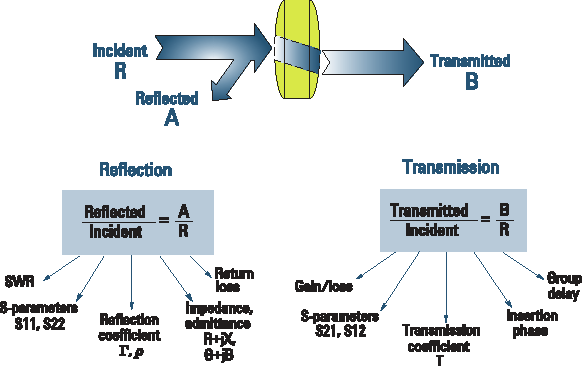
\includegraphics{img/analysis/vnaWaves.pdf}
    \caption{Fundamental Network Analyzer measurement \cite{agilentAppNoteVNA}.}
    \label{fig:vnaWaves}
\end{figure}

The essential component behind the Network Analyzer is the signal-separation hardware. This is used to separate the incident wave from the reflected wave in the test ports. The two separated waves can then be measured independently to get the phase and magnitude information \cite{nationalInstruVNA}. 

\subsection{Calibration}
In order to accurately measure the phase and magnitude of the incident and reflected waves, the VNA needs to be properly calibrated. Even though some elements of the VNA are calibrated at manufacturing, not everything can be accounted for. Different cables and connectors can have a large effect on the phase and magnitude and even a difference room temperature can affect the measurements \cite{nationalInstruVNA}. Due to all these variables, it is important to calibrate the VNA before a measurement.

\subsubsection{Sources of Error}
\label{sec:vnaerrorsource}
There are generally four inherent sources of error in the VNA. These are often referred to as systematic source of error due to their presence at all time, however they can all be greatly suppressed by calibration \cite{nationalInstruVNA}. These systematic sources of error at listed below: 
\begin{itemize}
\item Port match.
\item Directivity.
\item Frequency response.
\item Isolation.
\end{itemize}

\paragraph{Port match} Ideally, the VNA ports would have an input impedance of exactly \SI{50}{\ohm}. This is, however, hard to realize in reality and a small loss will be present at each port of the VNA due to mismatch \cite{nationalInstruVNA}.

\paragraph{Directivity} This source of error has its origin in the signal-separation hardware. The imperfections in these allow for a small portion of the reflected wave to leak into the reverse direction. Due to this finite isolation between the paths, the waves will not be perfectly separated. This can be compensated by the calibration \cite{nationalInstruVNA}. 

\paragraph{Frequency Response} Due to the multiple receivers which are inherently present in VNAs, lies a source of error. This is due to small differences in the frequency response in the receivers. The calibration of this is referred to as reflection and transmission tracking \cite{nationalInstruVNA}.
   
\paragraph{Isolation} Ideally, the VNA ports would be totally isolated, which is hard to realize in practice. This causes some of the measured signal at one port to leak into the other. This is also called cross-talk, and can be compensated by the calibration \cite{nationalInstruVNA}.

\subsection{Calibration Types}
There are multiple methods that can be used to calibrate a VNA. These depend on the number of ports, frequency range, and the device under test. However, for a two-port VNA, the following types are the most common:
\begin{itemize}
\item Frequency response calibration.
\item One-path two-port calibration.
\item Full $S$-parameter calibration.
\end{itemize}

\paragraph{Frequency Response Calibration} is the simplest method of calibration. It is sometimes termed transmission normalization. This only corrects the frequency response of the VNA, and should only be used when a rough measurement of $S_{12}$ and  $S_{21}$ is sufficient.
 
\paragraph{One-path Two-Port Calibration} allows for accurate forward $S$-parameter measurement. This type of calibration assumes that port two of the VNA is perfectly matched, and can therefore only be used for accurate $S_{11}$ and $S_{21}$.

\paragraph{Full $S$-Parameter Calibration} is the most complete calibration type since it takes all ports into account during the calibration. This allows for accurate measurements of all four $S$-parameters. There are multiple ways of doing a full two-port calibration, and the most common are the Short-Open-Load-Through (SOLT) method. For modern VNAs, electronic calibration standards are often used. 

\subsubsection{Short-Open-Load-Through}
This is a cheap and easy way of accurately calibrating a VNA. Basically, a set of known connectors with known values, which consist of a connector that is shorted, a connector that is open, a connector with a \SI{50}{\ohm} load, and lastly, the two cables are connected together with a female-female connector. The short and open circuit will create fully reflected voltage and current waves on the transmission line. The \SI{50}{\ohm} will result in full absorption, such that all the incident power is absorbed \cite{agilentAppNoteVNA}. Generally, the \SI{50}{\ohm} load is the source of error in these types of calibrations, since it is hard to get a perfect \SI{50}{\ohm} load in reality \cite{nationalInstruVNA}. 

\subsubsection{Electronic Calibration}
The electronic calibration kits are generally made by having a range of different known impedance states that are electronically switchable \cite{agilentEcal}. The characteristics are often stored in the calibration kit and can be read by the VNA. The calibration is similar to the SOLT method, but can support more complex impedance states \cite{agilentEcal}. 

\begin{aautail}
    In this section, the basic functionality of a VNA and the importance of calibrating has been described. This makes it possible to make accurate $S$-parameter measurements on the prototypes which will be designed in this project. In the next section, the functionality of the Satimo StarLab anechoic chamber will be described in order to show how efficiency and farfield measurement can be made as well.
\end{aautail}


%http://download.ni.com/evaluation/rf/Introduction_to_Network_Analyzer_Measurements.pdf VNA (\cite{nationalInstruVNA}
%http://cp.literature.agilent.com/litweb/pdf/5965-7707E.pdf VNA (\cite{agilentAppNoteVNA})

%http://cp.literature.agilent.com/litweb/pdf/5988-9477EN.pdf Ecal (\cite{agilentEcal})
